\documentclass[11pt]{article}
\usepackage[utf8]{inputenc} % Required for inputting international characters
\usepackage[T1]{fontenc} % Output font encoding for international characters
%TODO Decide between Palantino and Computer modern
\usepackage{mathpazo} % Palatino font
\usepackage{subfiles}
\usepackage{multirow}
\usepackage{amssymb}
\usepackage{amsmath}
\usepackage[margin=1in]{geometry}
\usepackage{enumitem}
\usepackage{caption}
\usepackage{graphicx} %package to manage images
\setlength{\emergencystretch}{10pt} % handles text going outside of boxes
\setcounter{tocdepth}{2} %makes the table of contents only go 2 layers deep
\usepackage[export]{adjustbox} % for frames on figures
\usepackage{multicol}
%TODO Decide if we want first paragraph tabbed after section
%\usepackage{indentfirst}
\begin{document}
%----------------------------------------------------------------------------------------
%	TITLE PAGE
%----------------------------------------------------------------------------------------
\begin{titlepage} % Suppresses displaying the page number on the title page and the subsequent page counts as page 1
	\newcommand{\HRule}{\rule{\linewidth}{0.5mm}} % Defines a new command for horizontal lines, change thickness here
	
	\center % Centre everything on the page
	
	%------------------------------------------------
	%	Headings
	%------------------------------------------------
	
	\textsc{\LARGE McGill University}\\[1.5cm] % Main heading such as the name of your university/college

	\textsc{\large COMP 551 - Applied Machine Learning}\\[0.5cm] % Minor heading such as course title
	
	%------------------------------------------------
	%	Title
	%------------------------------------------------
	
	\HRule\\[0.4cm]
	
	{\huge\bfseries Assignment 3 Report}\\[0.4cm] % Title of your document
	
	\HRule\\[1.5cm]
	
	%------------------------------------------------
	%	Author(s)
	%------------------------------------------------
	
	\begin{minipage}{0.5\textwidth}
		\begin{flushleft}
			\large
			Written by:\\
			Asher \textsc{Wright} - {\small 260559393}
		\end{flushleft}
	\end{minipage}
	~
	\begin{minipage}{0.4\textwidth}
		\begin{flushright}
			\large
			Due to:\\
			Prof.  \textsc{Chandar} 
		\end{flushright}
	\end{minipage}
	

	
	%------------------------------------------------
	%	Date
	%------------------------------------------------
	
	\vfill\vfill\vfill % Position the date 3/4 down the remaining page
	
	{\large February 26, 2018} 
		%----------------------------------------------------------------------------------------
	
	\vfill % Push the date up 1/4 of the remaining page
\end{titlepage}

\pagebreak
\section{Note about collaboration}
I discussed with Florence Regol RE which hyperparameters to tune, why, and what values we felt were important. No code or data was transferred.

\section{Note about F1 Measure}
The F1 measure was calculated using the method in the sklearn library. There are many different options for calculating F1 using this method, namely binary, micro, macro, weighted, and samples. For the binary bag of words, the average "binary" was used. For frequency bag of words, "micro" was used. The reason for using micro was because it seemed the closest to the binary version, as it acts by counting true positives, false negatives, and false positives.

\section{Raw F1 Measure Data}
Tables 1 and 2 show the raw F1 data for the classifiers, split by the two datasets.
\begin{table}[ht]
\centering
\caption{Yelp Classifier F1 Measures}
\label{my-label}
\begin{tabular}{llllll}
                                                 & Training F1 \%             & Validation F1 \%           & Testing F1 \% &  &  \\ \cline{1-4}
\multicolumn{1}{l|}{Random Classifier}           & \multicolumn{1}{l|}{20.03} & \multicolumn{1}{l|}{N/A}   & 20.55         &  &  \\
\multicolumn{1}{l|}{Majority Classifier}         & \multicolumn{1}{l|}{35.26} & \multicolumn{1}{l|}{N/A}   & 35.10         &  &  \\
\multicolumn{1}{l|}{BBoW: Bernoulli NB} & \multicolumn{1}{l|}{74.70} & \multicolumn{1}{l|}{42.50} & 44.25         &  &  \\
\multicolumn{1}{l|}{BBoW: Decision Tree}         & \multicolumn{1}{l|}{52.87} & \multicolumn{1}{l|}{39.10} & 39.40         &  &  \\
\multicolumn{1}{l|}{BBoW: Linear SVM}            & \multicolumn{1}{l|}{69.59} & \multicolumn{1}{l|}{48.50} & 43.55         &  &  \\
\multicolumn{1}{l|}{FBoW: Gaussian NB}  & \multicolumn{1}{l|}{80.25} & \multicolumn{1}{l|}{36.80} & 31.00         &  &  \\
\multicolumn{1}{l|}{FBoW: Decision Tree}         & \multicolumn{1}{l|}{39.64} & \multicolumn{1}{l|}{38.50} & 38.50         &  &  \\
\multicolumn{1}{l|}{FBoW: Linear SVM}            & \multicolumn{1}{l|}{60.84} & \multicolumn{1}{l|}{46.10} & \textbf{49.55}         &  & 
\end{tabular}
\end{table}

\begin{table}[ht]
\centering
\caption{IMDB Classifier F1 Measures}
\label{my-label}
\begin{tabular}{llllll}
                                         & Training F1 \%             & Validation F1 \%           & Testing F1 \% &  &  \\ \cline{1-4}
\multicolumn{1}{l|}{Random Classifier}   & \multicolumn{1}{l|}{50.49} & \multicolumn{1}{l|}{N/A}   & 49.59         &  &  \\
\multicolumn{1}{l|}{BBoW: Bernoulli NB}  & \multicolumn{1}{l|}{87.01} & \multicolumn{1}{l|}{84.26} & 82.98         &  &  \\
\multicolumn{1}{l|}{BBoW: Decision Tree} & \multicolumn{1}{l|}{87.55} & \multicolumn{1}{l|}{71.85} & 72.40         &  &  \\
\multicolumn{1}{l|}{BBoW: Linear SVM}    & \multicolumn{1}{l|}{98.96} & \multicolumn{1}{l|}{86.28} & \textbf{84.86}         &  &  \\
\multicolumn{1}{l|}{FBoW: Gaussian NB}   & \multicolumn{1}{l|}{86.11} & \multicolumn{1}{l|}{76.63} & 68.76         &  &  \\
\multicolumn{1}{l|}{FBoW: Decision Tree} & \multicolumn{1}{l|}{75.56} & \multicolumn{1}{l|}{68.79} & 71.08         &  &  \\
\multicolumn{1}{l|}{FBoW: Linear SVM}    & \multicolumn{1}{l|}{98.46} & \multicolumn{1}{l|}{83.91} & 83.48         &  & 
\end{tabular}
\end{table}
\section{Yelp Dataset}
Note that discussion about the performance of the classifiers will occur after all the data are reported.
\subsection{Common Classifiers}
The following two classifiers are independent of whether binary bag of words or frequency bag of words was used, since they do not take these data into consideration.

\subsubsection{Random Classifier}
The random classifier for the Yelp dataset had a Training F1 measure of 20.03\% and a Testing F1 measure of 20.55\%. Note that the validation performance was not measured for this classifier, since there is nothing to tune.

\subsubsection{Majority Classifier}
The majority Classifier for the Yelp dataset had a Training F1 measure of 35.26\% and a Testing F1 measure of 35.10\%.

\subsection{Binary Bag of Words}
The converted dataset for binary bag of words is included in the submitted files.

\subsubsection{Bernoulli Naive Bayes Classifier}
The hyperparameter that was cross-validated for Bernoulli Naive Bayes was alpha, which is the additive smoothing parameter. The closer to 0 alpha is, the less smoothing. The range of alpha examined was 1E-5 to 10. Figure 1 shows the F1 measure on the validation set versus alpha. One can see that there is a clear increase and decrease at the beginning of the range. The highest validation F1 measure of 42.50\% occurred when alpha = 0.01. This led to a training F1 measure of 74.70\% and a testing F1 measure of 44.25\%.

\begin{figure}[ht]
\centering
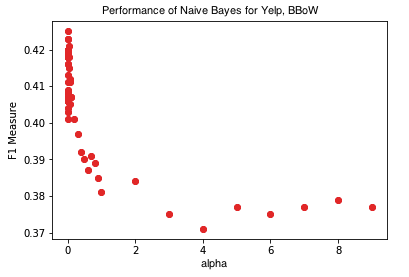
\includegraphics[width=0.65\textwidth]{Yelp_BernoulliNB}
\caption{F1 measure versus alpha for Bernoulli NB (Yelp)}
\end{figure}

\subsubsection{Decision Tree Classifier}
For the decision tree classifier, the only hyperparameter that was cross-validated was the maximum depth of the tree. This was discussed in lecture as a good parameter to validate. The range for this parameter was between 1 and infinity (covering 12 values). The highest validation F1 measure of 39.10\% occurred when the maximum depth was 10. This corresponded to a training F1 measure of 52.87\% and a testing F1 measure of 39.40\%.\\

\noindent
Figure 2 shows the performance relative to the maximum depth (infinite depth is not shown). One can see the early peak, followed by steady values.

\begin{figure}[ht]
\centering
\includegraphics[width=0.65\textwidth]{Yelp_DT}
\caption{F1 measure versus maximum depth for Decision Tree (Yelp)}
\end{figure}

\subsubsection{Linear SVM Classifier}
Three hyperparameters were cross-validated for linear SVM: tolerance, maximum iterations, and C (the penalty parameter of the error term). The tolerance for stopping and the penalty are important parameters to validate. The reason for validating the maximum iterations is to reduce overfitting. Without reducing the maximum iterations, the system almost always had near 100\% training accuracy, but low testing accuracy. The ranges of the parameters was as follows:
\begin{itemize}
\item tolerance: 1E-6 to 1E-4
\item C: 1E-1 to 1
\item maximum iterations: {1, 2, 5, 10}
\end{itemize}
Note that this range was found somewhat empirically, by adjusting the values and looking for changes. The highest validation F1 measure was 48.50\% and occurred when tolerance = 9E-5, maximum iterations = 2, and C = 0.5. This corresponded to a training F1 measure of 69.59\% and a testing F1 measure of 43.55\%. 

\subsection{Frequency Bag of Words}
The converted dataset for frequency bag of words is included in the submitted files.

\subsubsection{Gaussian Naive Bayes Classifier}
Since the frequency dataset is not binary, we switch to a Gaussian Naive Bayes classifier. There were no hyperparameters to tune for this classifier. The training F1 measure was 80.26\%, the validation F1 measure was 36.80\%, and the testing F1 measure was 31.00\%. 

\subsubsection{Decision Tree Classifier}
The same range of maximum depth was used as for binary bag of words. The best maximum depth was found to be 1, with a validation F1 measure of 38.50\%. This corresponded to a training F1 measure of 39.64\% and a testing F1 measure of 38.50\%. Again, we see an early peak in performance, similar to Figure 2 and Figure 4.

\subsubsection{Linear SVM Classifier}
Again, the same range of hyperparameters was used. The best F1 measure was 46.10\%, and occurred when tolerance = 1E-5, maximum iterations = 10, and C = 5. This corresponded to a training F1 measure of 60.84\% and a testing F1 measure of 49.55\%.

\section{IMDB Dataset}
\subsection{Common Classifier: Random Classifier}
The random classifier for IMDB had a 50.48\% training F1 measure and a 49.59\% testing F1 measure.

\subsection{Binary Bag of words}

\subsubsection{Bernoulli Naive Bayes Classifier}
See Figure 3 for the change in performance versus alpha. The peak is clear, and one can see that, again, past a certain value, the performance steadily decreases. The highest validation F1 measure of 84.26\% occurred when alpha = 0.06. This led to a training F1 measure of 87.01\% and a testing F1 measure of 82.98\%.

\begin{figure}[h]
\centering
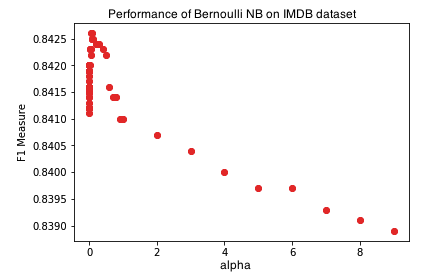
\includegraphics[width=0.65\textwidth]{IMDB_BernoulliNB}
\caption{F1 measure versus alpha for Bernoulli NB (IMDB)}
\end{figure}

\subsubsection{Decision Tree Classifier}
The best maximum depth was found to be 20, with a validation F1 measure of 71.85\%. This corresponded to a training F1 measure of 87.55\% and a testing F1 measure of 72.40\%.\\

\subsubsection{Linear SVM Classifier}
The best F1 measure was 86.28\%, and occurred when tolerance = 1E-6, maximum iterations = 10, and C = 0.1. This corresponded to a training F1 measure of 98.96\% and a testing F1 measure of 84.86\%.

\subsection{Frequency Bag of Words}
\subsubsection{Gaussian Naive Bayes Classifier}
The training F1 measure was 86.11\%, the validation F1 measure was 76.63\%, and the testing F1 measure was 68.76\%. 

\subsubsection{Decision Tree Classifier}
The best maximum depth was found to be 10, with a validation F1 measure of 68.79\%. This corresponded to a training F1 measure of 75.56\% and a testing F1 measure of 71.08\%.

\noindent
As with the other decision tree classifiers, we see an early peak in F1 measure relative to depth. This can be seen in Figure 4.

\begin{figure}[ht]
\centering
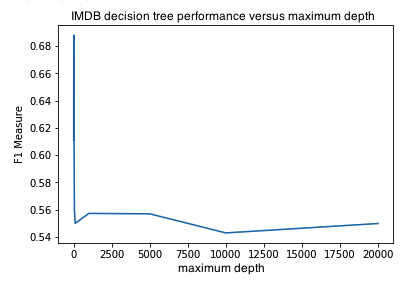
\includegraphics[width=0.65\textwidth]{IMDB_DT}
\caption{F1 measure versus maximum depth for Decision Tree (IMDB)}
\end{figure}

\subsubsection{Linear SVM Classifier}
The best F1 measure was 86.28\%, and occurred when tolerance = 1E-6, maximum iterations = 10, and C = 9. This corresponded to a training F1 measure of 98.46\% and a testing F1 measure of 83.48\%.

\section{Discussion}
For the Yelp Dataset with the Binary Bag of Words representation, The best performance (44.25\%) was the Bernoulli Naive Bayes. However, it was not far off from linear SVM (43.55\%). After switching to the Frequency Bag of Words representation, a more significant difference was noticed. There, Linear SVM performed the best by a significant margin (49.55\%). It's interesting to note that the decision tree classifier and Gaussian Naive Bayes performed worse than their binary bag of words counterparts. Overall, it seems like the frequency bag of words representation, paired with a cross-validated linear SVM is the best choice for the Yelp dataset.\\

This is not quite the case with the IMDB dataset. Here, we notice the same trends of the frequency bag of words representation classifiers performing worse for naive bayes and decision trees, but we also notice that it performs worse for the linear SVM, too. However, the decrease in F1 measure for the decision tree and SVM is much lower than that for Naive Bayes. The best performing classifier here is Linear SVM with the binary bag of words representation.\\

It is interesting that the best classifier for each dataset is a linear SVM, but with different representations. The reason that the frequency representation may be better for Yelp is because there are fewer words per review, whereas for IMDB the reviews are much longer, and thus binary suffices.\\

It is also interesting that we do not see a reliable improvement when using the frequency bag of words representation. I would have hypothesized that there would be an improvement, since it is just adding information for the classifier. However, it may be that we would need more data to take advantage of this extra information.\\

One further thing I would recommend doing is k-fold cross-validation, where, instead of using the same (and a single) validation set, different validation sets are created and tested. This could lead to a better classifier.

\end{document}